\section{Theorie}
\label{sec:Theorie}

Die Basis des Versuchs ist der photoelektrische Effekt, welcher den Austritt 
von Elektronen aus Anodenmaterial durch Lichtbestrahlung ermöglicht. Um das 
zu erklären, ist eine quantenmechanische Betrachtung notwendig.

\subsection{Licht als quantisierte Größe}
Die Auffassung von Licht als EM-Welle genügt nicht, um den Photoeffekt zu
erklären. Licht unterliegt dem Welle-Teilchen-Dualismus, was bedeutet, dass 
Licht quantisiert angesehen werden muss. Die Energie der quantisierten Ladung, 
dem Photon, ist über das Planck'sche Wirkungsquantum und die Frequenz verknüpft. 
Ersteres kann als universelle Konstante mit dem Wert $h = 6.626 \cdot 10^{-34} \unit{\joule\second}$
verstanden werden. Sie gibt an, dass Licht in diskreten Portionen aufgenommen 
oder abgegeben wird.
\begin{equation}
    \label{eqn:1}
    E = h \cdot \nu
\end{equation}
Wobei $\nu$ die Frequenz ist. Mithilfe dieser elementaren Gleichung wird erläutert,
dass die Energie eines Lichtquants zu einem Zeitpunkt nur absolut vollständig
an ein Elektron (beispielsweise in einer Anode) abgegeben werden kann.

\subsection{Photoeffekt an Metallen}
In diesem Experiment wird nur von Metallen ausgegangen, dessen Valenzelektronen 
frei beweglich sind. Diese sogenannten Fermionen unterliegen der Fermi-Dirac-
Verteilung, diese ist ein Maß für das thermische Gleichgewicht. Teilchen nahe 
der Fermi-Energie bzw. der Grenzfrequenz können die Anode verlassen. Um
zu ermöglichen, dass das Teilchen aus seinem gebundenen Zustand gelöst wird, muss Energie
hinzugefügt werden, es bedarf einer Austrittsarbeit $W_A$. Eine Möglichkeit
dafür ist die Bestrahlung mit monochromatischem Licht (mit der Energie aus
\autoref{eqn:1}). Für sie gilt (mit der Grenzfrequenz $\nu_G$)
\begin{equation}
    \label{eqn:2}
    W_A = h \cdot \nu_G
\end{equation}
Für Elektronen mit einer Energie größer der Austrittsarbeit, so haben die 
Teilchen eine zusätzliche Energie von $E_{kin} = \frac{1}{2} m v^2$, wodurch sich 
die Gesamtenergiebilanz als 
\begin{equation}
    \label{eqn:3}
    E = W_A + \frac{1}{2} m v^2
\end{equation}
schreiben lässt.
\vspace{0.5em}
\\
Für die Bestimmung der angesprochenen kinetischen Energie wird eine Photozelle 
genutzt, wie sie in \autoref{fig:1} zu sehen ist.
\begin{figure}[H]
    \centering
        \centering
        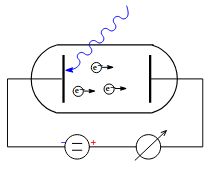
\includegraphics[width=0.5\textwidth]{Bilder/ggfeld.png}
        \caption{Gegenfeldmethode. \cite{anleitung9}}
    \hfill
    \label{fig:1}
\end{figure}
\noindent Das einfallende Licht der Energie $E= h \nu$ löst die Elektronen raus und
beschleunigt sie in Richtung der Anode, durch eine angelegte Gegenspannung $U_G$
werden diese allerdings verlangsamt bis sie die Anode schließlich nicht mehr 
erreichen. Folglich gilt der Energiezusammenhang
\begin{equation}
    \label{eqn:4}
    E = W_A + E_{el}
\end{equation}
mit der elektrischen Energie des Gegenfeldes $E_{el} = e_0 U_G$. Aufgelöst nach 
der Grenzspannung ergibt das
\begin{equation}
    \label{eqn:5}
    U_G = \frac{h \nu}{e_0} + W_A.
\end{equation}

\subsection{Fehlerrechnung}
Die gemessenen Werte unterliegen Messunsicherheiten und werden demnach im
Folgenden nicht als fehlerfrei angesehen. Die Fehler entstehen bei der
Bildung der Mittelwerte durch den Fehler des Mittelwerts und bei der
Regressionsrechnung sowie der Fehlerforpflanzung durch Python.
Der Mittelwert ist definiert durch
\begin{equation}
    \overline{x} = \frac{1}{N} \sum\limits_{i=1}^N x_i.
\end{equation}
\noindent Der Fehler des Mittelwerts ist somit gegeben durch 
\begin{equation}
    \begin{aligned}
        \increment \overline{x} &= \sqrt{\overline{x^2\kern-0.1em} - \overline{x}^2} \\
                            &= \frac{\sqrt{\frac{1}{N-1} \sum\limits_{i=1}^N (x_i - \overline{x})^2}}{\sqrt{N}}.
    \end{aligned}
\end{equation}

Um Fehler einzubeziehen, wird die Gauß'sche Fehlerfortpflanzung verwendet:
\begin{equation}
    \label{eqn:9}
    \increment f = \sqrt{\left(\frac{\partial f}{\partial x}\right)^2 \cdot \left(\increment x\right)^2 + \left(\frac{\partial f}{\partial y}\right)^2 \cdot \left(\increment y\right)^2 + .... + \left(\frac{\partial f}{\partial z}\right)^2 \cdot \left(\increment z\right)^2}
\end{equation}